\documentclass{amsart}
\usepackage{graphicx,amsmath,tikz,biblatex} % Required for inserting images
\addbibresource{bib.bib}
\title{Project 5: Predator-prey Model}
\author{Gabriel Arteaga}
\date{November 2024}

\begin{document}
\begin{abstract}
    This paper explores the dynamics of predator-prey interactions alongside the context of harvesting, using the Lotka-Voletrra model as a starting point. We examine how overfishing can affect the stability of these populations by introducing harvesting rates for both predator and prey species. We use phase plots of the system to conclude that harvesting activities can destabilize populations and potentially lead to the extinction of populations, or maintain equilibrium with controlled harvesting. We extend our system to three populations and conclude that the harvesting of predator populations can potentially lead to population decline. Historical context, including D'Anacona's data and the conclusions of \textit{Cascading Effects of the Loss of Apex Predatory Sharks from a Coastal Ocean}, is incorporated to highlight the careful balance of harvesting and population, and what may occur if this balance is not kept. 
\end{abstract}
\maketitle

\section{Introduction}
Predator-prey models are a cornerstone of differential equations research, offering valuable insights into biology, ecology, and related disciplines. By studying how populations interact, we gain the ability to address critical issues such as population collapse due to overhunting. This was the motivation behind Vito Volterra's work in 1927 after Umberto D'Ancona presented intriguing wartime data: during World War I, selachian fish populations experienced a noticeable spike. Volterra developed his model, expanding upon Pierre-François Verhulst's earlier work, to explain this phenomenon. Soon after, Alfred Lotka contacted Volterra, pointing out that elements of this analysis had appeared in Lotka's 1925 publication. Consequently, the model became known as the Lotka-Volterra equations, which serve as the starting point for our analysis.


In Section~\ref{sec:Pred-prey} we expand the Lotka-Volterra equation to account for overcrowding, then through qualitative analysis understand the system's equilibrium and its phase plot. Section~\ref{sec:Fishermen} introduces two terms to our system to understand what happens when we harvest portions of the population, using the same type of qualitative analysis. We then compare the two systems to understand the effects of harvesting on the populations. Finally in Section~\ref{sec:Trophic-Cascading} analyze a three-population model to confirm the data presented in \textit{Cascading Effects of the Loss of Apex Predatory Sharks from a Coastal Ocean} by looking at the derivative of stable equilibria of this system.

\section{Predator-Prey Model}\label{sec:Pred-prey}
We begin this model by defining a population system with $x(t)$, our prey population, and $y(t)$ our predator population, their per capita growth rate will be,
\begin{equation*}
    \left\{
    \begin{aligned}
        &\frac{dx/dt}{x}=a_1\\
        &\frac{dy/dt}{y}=-a_2.
    \end{aligned}
    \right.
\end{equation*} 
Without species interaction, the prey will populate due to a lack of predatory pressure, and the predators will starve. Considering the interaction of these species, we consider a deduction from the prey population by a factor of $b_{12}$ as the predators hunt their population. Conversely, this allows the predators to hunt, which increases predator population by a factor of $b_{21}$. This leads to our system becoming, 
\begin{equation*}
    \left\{
    \begin{aligned}
        &\frac{dx/dt}{x}=a_1-b_{12}y\\
        &\frac{dy/dt}{y}=-a_2+b_{21}x.
    \end{aligned}
    \right.
\end{equation*} 
This system is the Lotka-Volterra model published in $1926$~\cite{volterra1926fluctuations}, however, we will consider one more term, which comes in the form of overcrowding. This leads to a decrease in both populations, in factors of $b_{11}$ for the prey and $b_{22}$ for the predators. This makes our system, 
\begin{equation*}
    \left\{
    \begin{aligned}
        &\frac{dx/dt}{x}=a_1-b_{12}y-b_{11}x\\
        &\frac{dy/dt}{y}=-a_2+b_{21}x-b_{22}y.
    \end{aligned}
    \right.
\end{equation*}
Rewriting for our rate of change of each population gives us, 
\begin{equation}\label{eq:sys-1}
    \left\{
    \begin{aligned}
        &\frac{dx}{dt}=x(a_1-b_{12}y-b_{11}x)\\
        &\frac{dy}{dt}=y(-a_2+b_{21}x-b_{22}y).
    \end{aligned}
    \right.
\end{equation}
This formulation presents the issue that this system is non-linear, so we rely on qualitative analysis. To do so we first find all four equilibria of our system, the first of which comes when we set both $y=0$ and $x=0$, no starting population at all, this gives
\begin{align*}
    E_{1a}= \{y=0,\, x=0\}.
\end{align*}
Our next two equilibria are based on solutions for the equations of our prey and predator nullclines. These equations are, 
\begin{align*}
    &a_1-b_{12}y-b_{11}x=0,\\
    -&a_2+b_{21}x-b_{22}y=0.
\end{align*}
We get our second equilibrium by setting $y=0$ and solving the prey nullcline equation, the first equation, for $x$, this gives,
\begin{align*}
    E_{2a}=\left\{y=0,\, x=\frac{a_1}{b_{11}}\right\}.
\end{align*}
We get our third equilibrium from setting $x=0$ and solving for our predator nullcline equation, the second equation, for $y$, this gives,
\begin{align*}
    E_{3a}=\left\{y=\frac{-a_2}{b_{22}},\, x=0\right\}.
\end{align*}
Our final equilibrium is,
\begin{align*}
    E_{4a}=\left\{
x = \frac{a_1 b_{22} + a_2 b_{12}}{b_{11} b_{22} + b_{12} b_{21}}, \quad
y = \frac{a_1 b_{21} - a_2 b_{11}}{b_{11} b_{22} + b_{12} b_{21}}
\right\}
\end{align*}
We now plot these equilibrium points, beginning by plotting the origin equilibrium, $E_{1a}$, a point at the equilibrium. We then plot the prey nullcline, this enters the first quadrant at $\left(0,\frac{a_1}{b_{12}}\right)$, and exits at $\left(\frac{a_1}{b_{11}},0\right)$, this point is $E_{2a}$. Then, we plot the predator nullcline, this line enters the fourth quadrant at, $\left(0,\frac{-a_2}{b_{22}}\right)$, this is $E_{3a}$. It then enters the first quadrant at$\left(\frac{a_2}{b_{21}},0\right)$ and extends infinitely upwards and to the right. Finally, we arrive at the intersection of the two nullclines, $E_{4a}$, we will find that this equilibrium is our stable equilibrium. A graph with all nullclines and equilibrium points is plotted in figure~\ref{fig:tikz2}.\\

To see how our phase plot will look we consider a point near $E_1$, this is an unstable equilibrium as such the population moves away from this point and toward the prey nullcline. As it approaches this nullcline $\frac{dy}{dt}$ approaches $0$, as such when it crosses this line it will cross horizontally. The population continues this path until it reaches the predator nullcines, where $\frac{dx}{dt}$ becomes $0$. However at the same time, it gets closer to $E_2$, another unstable equilibrium, as such it moves vertically away from this point. After this, it reaches the prey nullcline again once again crossing it horizontally, then the predator nullcline again vertically. This continues, each pass-through getting closer to $E_{4a}$ in a spiraling manner until it converges to this stable equilibrium. We plot this behavior in Maple, but we must first choose some arbitrary parameters, 
\begin{align*}
   a= \begin{bmatrix}
        4\\
        1
    \end{bmatrix}
    ,\, B=\begin{bmatrix}
        1 & 1& 1\\
        1 & 1 & 1
    \end{bmatrix}.
\end{align*}
Plotting this in Maple we see this expected convergence, as shown in figure~\ref{fig:phaseplot1}. However, we have made a critical assumption here, namely $\frac{a_1}{b_{11}}>\frac{a_2}{b_{21}}$. Suppose we reverse this inequality and choose our parameters as 
\begin{align*}
   a= \begin{bmatrix}
        1\\
        4
    \end{bmatrix}
    ,\, B=\begin{bmatrix}
        1 & 1& 1\\
        1 & 1 & 1
    \end{bmatrix}. 
\end{align*}
Plotting our new system in Maple gives us figure~\ref{fig:phaseplot-3}, we now see our nullclines intersect below the first quadrant. Additionally, our stable and unstable equilibria have changed, $E_{2a}$ is our new stable equilibrium. As this equilibrium is missing a population this then implies that no matter what our predator population dies out. This does not correspond with reality, and as such we will choose our previous assumption to analyze for the rest of this paper.
\begin{figure}
    \centering
    \includegraphics[width=0.5\linewidth]{phaseplot1.png}
    \caption{Phase plot of system~\eqref{eq:sys-1}, with the assumption that $\frac{a_1}{b_{11}}>\frac{a_2}{b_{21}}$. Overlaid are the predator and prey nullclines.}
    \label{fig:phaseplot1}
\end{figure}
\begin{figure}
    \centering
    \begin{tikzpicture}[> =latex]
        \coordinate (E0) at (0,0);
        \coordinate (E1) at (4,0);
        \coordinate (F1) at (0,4);
        \coordinate (E2) at (0,-1);
        \coordinate (F2) at (4,3);
        \coordinate (E3) at (5/2, 3/2);
        \draw[green] (E1) -- (F1); %prey line
        \draw[red] (E2) -- (F2); %predator line
        \draw[->] (0,0) -- (5,0) node[below] {$x$};
        \draw[->] (0,-1.6) -- (0,5) node [right] {$y$};
        %\draw[green,dashed] (3.5,0) -- (0,3.5); %this needs to be fixed
        %\draw[red, dashed] (0,-1.5) -- (4,2.5); %this also needs fixing
        \fill[blue] (E0) circle (0.1);
        \fill[blue] (E1) circle (0.1);
        \fill[blue] (E2) circle (0.1);
        \fill[blue] (E3) circle (0.1);
        \node[below=0.4ex] at (E1) {$\frac{a_1}{b_{1,1}}$};
        \node[right= 0.4ex] at (E2) {$-\frac{a_2}{b_{2,2}}$};
        %\fill[blue] (2.5,1) circle (0.1);
    \end{tikzpicture}
    \caption{This shows all equilibrium points of system~\eqref{eq:sys-1}. The line in green is the predator nullcline, and the line in red is the prey nullcline.}
    \label{fig:tikz2}
\end{figure}

\begin{figure}
    \centering
    \includegraphics[width=0.5\linewidth]{phaseplot3.png}
    \caption{Phase plot of system~\eqref{eq:sys-1} with the assumption that $\frac{a_1}{b_{11}}<\frac{a_2}{b_{21}}$. }
    \label{fig:phaseplot-3}
\end{figure}


\section{Fishing}\label{sec:Fishermen}
We now introduce two terms to account for the impact of fishing. The first term $\alpha x$ represents the harvesting of the prey population, where $\alpha$ reflects the factor of removal due to fishing. Similarly, the second term $\beta y$ models the harvesting of the predator population, where $\beta$ represents the factor of removal either due to direct fishing or bycatch. Incorporating these to system~\eqref{eq:sys-1} gives, 
\begin{equation}\label{eq:sys-2}
    \left\{
    \begin{aligned}
        &\frac{dx}{dt}=x(a_1-b_{11}x-b_{12}y)-\alpha x\\
        &\frac{dy}{dt}=y(-a_2-b_{22}y+b_{21}x)-\beta y.
    \end{aligned}
    \right.
\end{equation}
How does this contextually change our system? System~\eqref{eq:sys-1} modeled the spike in D'Anacona's data during World War $1$, when fishing was restricted. The inclusion of harvesting terms in system~\eqref{eq:sys-2} allows us to study the periods before and after the spike. We will confirm this by qualitatively analyzing the system and seeing the differences in the new phase plot. We begin by noticing that the system still is not linear. As such we begin by finding the equilibria once more, starting with the origin equilibrium we attain,
\begin{equation*}
          E_{1b}=\left\{
    \begin{aligned}
    y=0,\, x=0    
    \end{aligned}
   \right\}.
\end{equation*}
Our nullcline equations are, 
\begin{align*}
    &a_1-b_{12}y-b_{11}x-\alpha=0,\\
    -&a_2+b_{21}x-b_{22}y-\beta=0.
\end{align*}
Our second equilibrium comes from setting $x=0$ and solving for $y$ in the second nullcline equation, this gives,
\begin{align*}
    E_{2b}=\left\{
    \begin{aligned}
    y=-\frac{a_2+\beta}{b_{22}},\, x=0    
    \end{aligned}
   \right\}.
\end{align*}
Our third equilibrium comes from setting $y=0$ and solving for $x$ in the first nullcline equation, this gives,
\begin{align*}
    E_{3b}=\left\{
    \begin{aligned}
    y=0,\, x=\frac{a_1-\alpha}{b_{11}}    
    \end{aligned}
   \right\}.
\end{align*}
Much like our last system, our final equilibrium comes from setting $\frac{dx}{dt}$ and $\frac{dy}{dt}$ to zero, and solving for $x$ and $y$. This gives us,
\begin{align*}
    E_{4b}=\left\{
    y = \frac{a_1 b_{21} - a_2 b_{11} - \alpha b_{21} - \beta b_{11}}{b_{11} b_{22} + b_{12} b_{21}} , \quad 
x = \frac{a_1 b_{22} + a_2 b_{12} - \alpha b_{22} + \beta b_{12}}{b_{11} b_{22} + b_{12} b_{21}}
    \right\}.
\end{align*}
We now plot these equilibrium points with the inclusion of the fishing effects. We first plot $E_{1b}$, which corresponds to a point at the origin. Our second equilibrium, $E_{2b}$ is the prey nullcline, it enters the first quadrant at $\left(0,\frac{a_1-\alpha}{b_{12}}\right)$ and leaves at $\left(\frac{a_1-\alpha}{b_{11}},0\right)$. Our third equilibrium $E_{3b}$ is the predator nullcline, it enters the first quadrant at $\left(\frac{a_2+\beta}{b_{21}},0\right)$ and extends infinitely upwards. Our final equilibrium is $E_{4b}$ the nullcline intersection, for this system it is still in the first quadrant but shifted downwards, additionally it is still our stable equilibrium. This system's equilibria are portrayed in figure~\ref{fig:tikz3}. Just as in the previous section we want to plot the phase plot of this system, using the same parameters for $a$ and $B$ we choose two arbitrary parameters for our harvesting, 
\begin{align*}
    \alpha=0.3,\, \beta=0.2.
\end{align*}
Figure~\ref{fig:phaseplot2} shows the new phase plot and as expected, the equilibria are shifted downwards due to the harvesting terms. To make a more concrete argument we draw lines from the origin to each of the nullcline intersections in both systems. We calculate the slope of the first system that gives us a wartime slope of, 
\begin{align*}
    m_a=\frac{3/2}{5/2}=\frac{3}{5}.
\end{align*}
Calculating the slope of the second intersection gives us a peacetime slope of, 
\begin{align*}
    m_b=\frac{5/4}{49/20}=\frac{25}{49}.
\end{align*}
Comparing the wartime and peacetime slopes confirms that the inclusion of fishing terms shifts the equilibria and impacts population dynamics. This implies an increase in the selachian population during periods of restricted fishing. This aligns with D'Ancona's data from 1914 to 1924, where a spike in the Selachian population occurred during World War $1$ due to limited fishing activities. The system shows this behavior with the downward shift in equilibria caused by harvesting, as seen in Figure~\ref{fig:phaseplot2}. During wartime, fishing restrictions effectively reduced the harvesting rate creating system~\eqref{eq:sys-1}, allowing predator and prey populations to stabilize at higher levels. In contrast, peacetime equilibria, system~\eqref{eq:sys-2}, reflect lower population levels due to active harvesting.

\begin{figure}
    \centering
    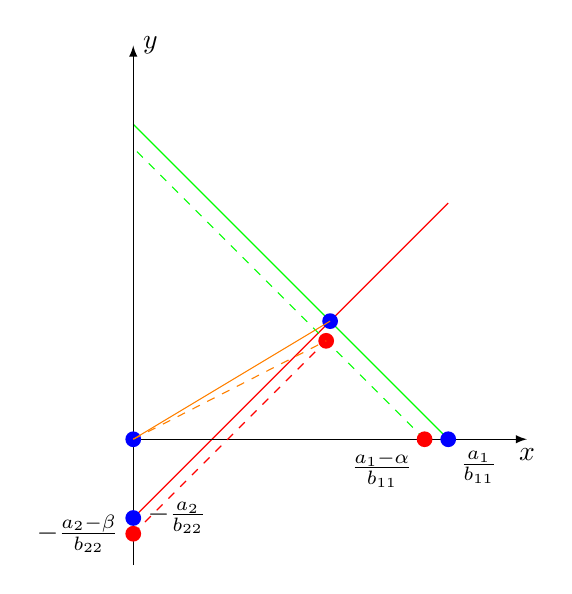
\begin{tikzpicture}[> =latex]
        \coordinate (E0) at (0,0);
        \coordinate (E1) at (4,0);
        \coordinate (F1) at (0,4);
        \coordinate (E2) at (0,-1);
        \coordinate (F2) at (4,3);
        \coordinate (E3) at (5/2, 3/2);
        \coordinate (E4) at (2.45,1.25);
        \draw[green] (E1) -- (F1); %prey line
        \draw[red] (E2) -- (F2); %predator line
        \draw[->] (0,0) -- (5,0) node[below] {$x$};
        \draw[->] (0,-1.6) -- (0,5) node [right] {$y$};
        \draw[green,dashed] (3.7,0) -- (0,3.7); %this needs to be fixed
        \draw[red, dashed] (0,-1.2) -- (E4); %this also needs fixing
        \fill[blue] (E0) circle (0.1);
        \fill[blue] (E1) circle (0.1);
        \fill[blue] (E2) circle (0.1);
        \fill[blue] (E3) circle (0.1);

        \fill[red] (E4) circle (0.1);
        \fill[red] (3.7,0) circle (0.1);
        \fill[red] (0,-1.2) circle (0.1);
        \node[below right=0.2ex] at (E1) {$\frac{a_1}{b_{11}}$};
        \node[below left=0.2ex] at (3.7,0) {$\frac{a_1-\alpha}{b_{11}}$};
        \node[right= 0.4ex] at (E2) {$-\frac{a_2}{b_{22}}$};
        \node[left=0.4ex] at (0,-1.2) {$-\frac{a_2-\beta}{b_{22}}$};
        \draw[orange,dashed] (0,0) -- (E4);
        \draw[orange] (0,0) -- (E3);


    \end{tikzpicture}
    \caption{This shows all equilibrium points from both of our systems. The lines in green are the predator nullclines, and the lines in red are the prey nullclines. Our old equilibria are represented in blue, while our new equilibria are represented in red. It shows the shift downward harvesting causes to the populations.}
    \label{fig:tikz3}
\end{figure}
\begin{figure}
    \centering
    \includegraphics[width=0.5\linewidth]{danacondadata.png}
    \caption{This plot shows D'Ancona's data of the Selachian population from $1914$ to $1924$.}
    \label{fig:danacondadata}
\end{figure}
\begin{figure}
    \centering
    \includegraphics[width=0.5\linewidth]{phaseplot2.png}
    \caption{This is the phase plot of the second system and has our equilibria and nullclines overlayed.}
    \label{fig:phaseplot2}
\end{figure}
\section{Trophic Cascading}\label{sec:Trophic-Cascading}
We now aim to extend our system into three populations to confirm the conclusion of \textit{Cascading Effects of the Loss of Apex Predatory Sharks from a Coastal Ocean} which suggested that if an increase in shark harvesting leads to a decrease in scallop population. We begin by creating a new system, we let $x(t)$ be our scallop population, $y(t)$ our ray population, and $z(t)$ our shark population. Without any species interaction, the per capita growth rate will be,
\begin{equation*}
    \left\{
 \begin{aligned}
    &\frac{dx/dt}{x}=a_1\\
    &\frac{dy/dt}{y}=a_2\\
    &\frac{dz/dt}{z}=-a_3.
\end{aligned}
\right.
\end{equation*}
We now consider the overcrowding factor which gives us, 
\begin{equation*}
    \left\{
 \begin{aligned}
    &\frac{dx/dt}{x}=a_1-b_{11}x\\
    &\frac{dy/dt}{y}=a_2-b_{22}y\\
    &\frac{dz/dt}{z}=-a_3-b_{33}z .
\end{aligned}
\right.
\end{equation*}
Next, we consider interspecies interaction, the rays will eat the scallops, negatively affecting the scallop population and positively affecting the ray population. The same is true for the ray and shark interaction. The sharks eat the rays, negatively affecting the ray population but benefiting the shark population. Note that there is no interaction between sharks and scallops. This gives us, 
\begin{equation*}
    \left\{
 \begin{aligned}
    &\frac{dx/dt}{x}=a_1-b_{11}x-b_{12}y\\
    &\frac{dy/dt}{y}=a_2-b_{22}y+b_{21}x-b_{23}z\\
    &\frac{dz/dt}{z}=-a_3-b_{33}z+b_{32}y .
\end{aligned}
\right.
\end{equation*}
Finally, we add our harvesting rates and solve for our differential equations. Our system becomes, 
\begin{equation} \label{eq:tri-sys}
    \left\{
 \begin{aligned}
    &\frac{dx}{dt}=x(a_1-b_{11}x-b_{12}y)-\alpha x\\
    &\frac{dy}{dt}=y(a_2-b_{22}y+b_{21}x-b_{23}z)- \beta y\\
    &\frac{dz}{dt}=z(-a_3-b_{33}z+b_{32}y)- \gamma z .
\end{aligned}
\right.
\end{equation}
As has happened with our previous two systems, this system is non-linear. As such we rely once more on qualitative analysis, beginning by finding our equilibria. There are eight total equilibria, and all but one of the equilibria contains missing populations, as such they are inconsistent with reality and not useful for our purposes. The final equilibrium however contains all three populations and is our stable equilibrium, it is shown below,
 
\begin{equation*}
    \left\{
    \begin{aligned}
      &x= \frac{\big((-a_2 + \beta)b_{12} + b_{22}(a_1 - \alpha)\big)b_{33}+b_{23}\big((-a_3 - \gamma)b_{12} + b_{32}(a_1 - \alpha)\big)}{\left(b_{11}b_{22} + b_{12}b_{21}\right)b_{33} + b_{11}b_{23}b_{32}},\\
        &y =\frac{\big((a_2 - \beta)b_{33} + b_{23}(a_3 + \gamma)\big)b_{11} + b_{33}b_{21}(a_1 - \alpha)}{\left(b_{22}b_{33} + b_{23}b_{32}\right)b_{11} + b_{12}b_{21}b_{33}}, \\
        &z = \frac{\big((a_2 - \beta)b_{32} - b_{22}(a_3 + \gamma)\big)b_{11} + b_{21}\big(b_{32}(a_1 - \alpha) - b_{12}(a_3 + \gamma)\big)}{\left(b_{22}b_{33} + b_{23}b_{32}\right)b_{11} + b_{12}b_{21}b_{33}}
    \end{aligned}
    \right\}.
\end{equation*}
With this equilibrium, we aim to see how changing the shark population will affect the ray and scallop populations. A positive change in the ray population will lead to overhunting of the scallop population, eventually leading to a collapse in the scallop population. Taking the derivative of our ray population in this equilibrium with respect to the shark harvesting rate, $\gamma$, will give us,

\begin{align*}
    \frac{dy}{d\gamma}=\frac{b_{11} b_{23}}{b_{11} b_{22} b_{33} + b_{11} b_{23} b_{32} + b_{12} b_{21} b_{33}}.
\end{align*}
This is a positive value, and as such infer that an increase in shark harvesting will only lead to an increase in the ray population. This leads to a sharp decline in the scallop population as more rays must satiate their hunger with scallops. We confirm this inference by taking the derivative of the scallop population in this equilibrium with respect to the shark harvesting rate, $\gamma$, this gives, 
\begin{align*}
    \frac{dx}{d\gamma}=\frac{-b_{12} b_{23}}{b_{11} b_{22} b_{33} + b_{11} b_{23} b_{32} + b_{12} b_{21} b_{33}}
\end{align*}
As we suspected this quantity is negative, telling us that any change in the shark population will eventually lead to a decrease in the scallop population. As mentioned in \textit{Cascading Effects of the Loss of Apex Predatory Sharks from a Coastal Ocean} this has catastrophic consequences, in $2004$ there was a century-old scallop fishery that was forced to close entirely due to a lack of scallop population surviving into the fall due to over predation by clown-nosed rays~\cite{science:sharks}.   


\section{Conclusion}
In this paper, we examined the dynamics of predator-prey interactions in the context of harvesting. The results show that overfishing of any of the populations can have a significant impact on the stability of all populations, leading to possible extinction. We began with the Lokta-Volterra model and introduced harvesting terms into the model, we observed how fishing affects both predator and prey populations, shifting the equilibria and changing the phase plot of the system. We specifically confirmed that as seen in D'Anacona's data, a lack of harvesting can lead to the stabilization of predator populations. We then extended our system to three populations and confirmed the findings of data from \textit{Cascading Effects of the Loss of Apex Predatory Sharks from a Coastal Ocean}, showing that a change in predator populations will always lead to a decline in a prey population. 




\printbibliography
\end{document} 